Insieme alla entità del gioco, ho iniziato a realizzare un semplice sistema di coordinate per gestire movimenti nell'arena, tenendo conto delle premesse fatte in fase di design:
\begin{itemize}
    \item la mappa di gioco deve essere rappresentata logicamente da una griglia;
    \item la mappa di gioco deve avere un contorno non attraversabile (\textit{Wall}) e un'area di gioco interna (\textit{Floor});
    \item ogni entità all'interno dell'arena è caratterizzata da una posizione (\textit{Position});
    \item ogni posizione si compone di un punto 2D (\textit{Point}) e di una direzione opzionale (\textit{Option[Direction]});
    \item ogni entità può muoversi solo in quattro direzioni;
    \item le coordinate possono essere solo numeri interi positivi.
\end{itemize}

Ho poi partecipato all'implementazione della classe \textit{Arena}, contenente tutte le entità che popolano la mappa durante il gioco. Alcuni componenti, vista la loro natura statica, vengono inizializzati con le loro posizioni in fase di creazione, mentre il resto viene gestito dalle funzioni \textit{generateMap()} e \textit{updateMap()}. Si noti la differenza tra \textit{Player}, che rappresenta l'utente, e \textit{Hero}, che invece rappresenta il personaggio giocabile. La classe ha come parametri il nome del profilo associato alla partita corrente ed un \textit{MapGenerator}, a sua volta inizializzato con la difficoltà della partita.

\begin{figure}[H]
  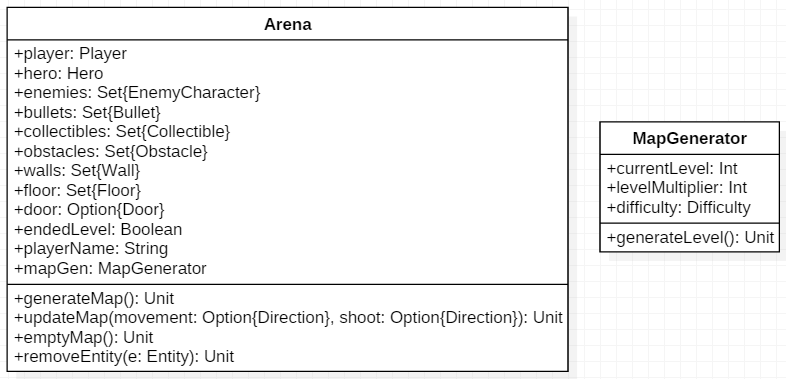
\includegraphics[width=14cm]{res/arenaClass.png}
  \caption{La classe \textit{Arena}}
  \label{arenaCLass}
\end{figure}

Vista l'importanza logica di \textit{Arena}, è anche necessario fornire metodi esterni generici per permettere alle altre classi di lavorare con l'area di gioco. Per lo scopo, un companion object contiene tutti i metodi che possono essere utili alle entità esterne per controllare lo stato del gioco, nonchè per il testing. Una parte fondamentale dello sviluppo è stata la scelta del tipo di funzioni da implementare in questo caso, che ha portato a refactoring in parti diverse dell'implementazione, dovuto soprattutto alla separazione tra funzioni della classe e del companion object e a scelte legate alle strutture dati utilizzate.

\begin{figure}[H]
  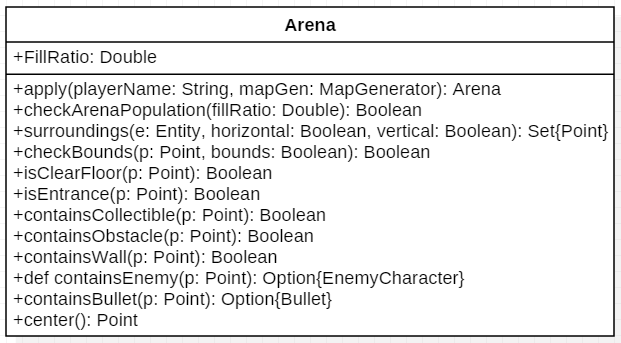
\includegraphics[width=14cm]{res/arenaObject.png}
  \caption{Il companion object di \textit{Arena}}
  \label{arenaObject}
\end{figure}